\chapter{Das Referenzmodell: Einzelne Kugel auf festem Grund}



\section{Erstellung und Equilibrierung der Probe}
	Eine Probe im Sinne der MD ist eine Datei, welche mindestens alle notwendigen Eigenschaften
	aller Teilchen im System speichert. Dazu gehören natürlich der Ort und die Geschwindigkeit
	jedes Teilchens, aber auch der Teilchentyp und die Teilchenmasse. Der Mulde im LJ-Potential
	\eqref{eq:potential_lj} nach gibt es für alle Teilchen einen Zustand minimaler Energie.
	Aus diesem Grund existiert ein stationärer Gleichgewichtzustand (\emph{Equilibrium}). Den
	Gesetzen der Thermodynamik folgend geht jedes ungestörte Nichtgleichgewichtssystem in sein
	Equilibrium über. Dieser Vorgang heißt \emph{Equilibrierung}. Da eine Probe prinzipiell einen
	beliebigen Zustand haben kann, ist eine \emph{vorherige} Equilibrierung besonders wichtig.
	Andernfalls findet der Equilibrierungsprozess gestört während der eigentlichen Simulation
	statt, was zu verfälschten Ergebnissen führen kann.

	Für das Modell dieser Arbeit bietet es sich an, eine auf \SI{300}{\kelvin} aufgeheizte Probe
	zu betrachten. Viele der in der Literatur auffindbaren Vergleichswerte zu Materialkonstanten
	werden bei diesem der Raumtemperatur nahe gelegenen Wert angegeben. Zudem bildet diese
	Temperatur das Problem gut ab.

	\subsection{Homogene Deformation}
		Um eine Probe nun in ihren Gleichgewichtszustand mit dieser Temperatur zu versetzen bietet
		es sich an, zuerst eine Probe der Temperatur \SI{0}{\kelvin} zu erstellen und diese dann
		aufzuheizen. Der rechnerische Nullpunkt lässt sich einfach dadurch erreichen, dass die
		Teilchengeschwindigkeiten auf 0 gesetzt werden. Mithilfe einer homogenen Deformation wird
		eine Simulation ohne Berücksichtigung der durch die Kraft verursachten Teilchenbewegungen
		durchgeführt. In jedem Simulationsschritt wird die Probe mithilfe einer zum Gitter
		achsenparallel wirkenden Deformationsmatrix inkrementell skaliert. Der sich dadurch
		ergebende Verlauf der mittleren potentiellen Energie kann nun minimiert werden. Aufgrund
		der Proportionalität zwischen dem Druck und den gemittelten Kräften äußert sich diese
		Stelle in Abbildung \ref{fig:homdef} in Form einer Nullstelle genau dort, wo die
		potentielle Energie minimal ist. Dies ist auch in sofern einleuchtend, da der Druck
		angibt, inwiefern sich einen Probe beim loslassen zusammenziehen oder ausdehnen würde
		\cite{rapp2014laserablation}.

		\begin{figure}[!ht]
			\centering
			\includegraphics[width=0.9\textwidth]{chapter/main/single/plt/equilibration/homdef.eps}
			\caption{Die mittlere potentielle Energie und der Probendruck aufgetragen gegen das
			Volumen pro Teilchen. Das Energieminimum kann durch einen näherungsweise quadratischen
			Fit um das Minimum der potentiellen Energie oder über eine Nullstellensuche des Druck
			bestimmt werden. In diesem Fall liegt das Energieminimum bei einem Teilchenvolumen von
			\SI{16.38}{\angstrom\cubed}.}
			\label{fig:homdef}
		\end{figure}

	\subsection{Aufheizen der Probe}
		Die bisherige Simulation fand unter Beachtung der Regeln eines mikrokanonischen Ensembles
		(\emph{NVE}) statt. Das bedeutet, dass neben der Teilchenzahl $N$ und dem Volumen $V$ die
		Gesamtenergie $E$ festgehalten wurde. Da im nächsten Schritt eine Temperaturerhöhung zum
		Aufheizen der Probe notwendig ist, ist ein NVE-Ensemble System so zwangsläufig ungeeignet.
		Stattdessen bietet sich das kanonische Ensemble (\emph{NVT}) an. Hier werden auch die
		Teilchenzahl und das Volumen fest gesetzt, allerdings wird hier statt der Energie die
		Temperatur $T$ durch Kopplung an ein Wärmebad vorgegeben. In der Simulation wird dies
		mithilfe eines Thermostats realisiert. Ein Thermostat manipuliert dabei die Simulation in
		der Hinsicht, dass die Temperatur der Vorgabe entspricht. Ein einfacher Thermostat wäre
		das Berendsen-Thermostat, bei dem der durch das Äquipartitionstheorem
		\eqref{eq:equipartition} gegebene Zusammenhang zwischen Temperatur und
		Teilchengeschwindigkeit genutzt wird, um alle Teilchengeschwindigkeiten global zu
		reskalieren. Dies hat allerdings einen Verlust der Maxwell-Boltzmann-Verteilung der
		Geschwindigkeitsbeträge zur Folge. Der in IMD verwendete Thermostat ist deshalb das
		\emph{Nosé-Hoover-Thermostat} \cite{rapp2014laserablation}.

		\begin{figure}[!ht]
			\centering
			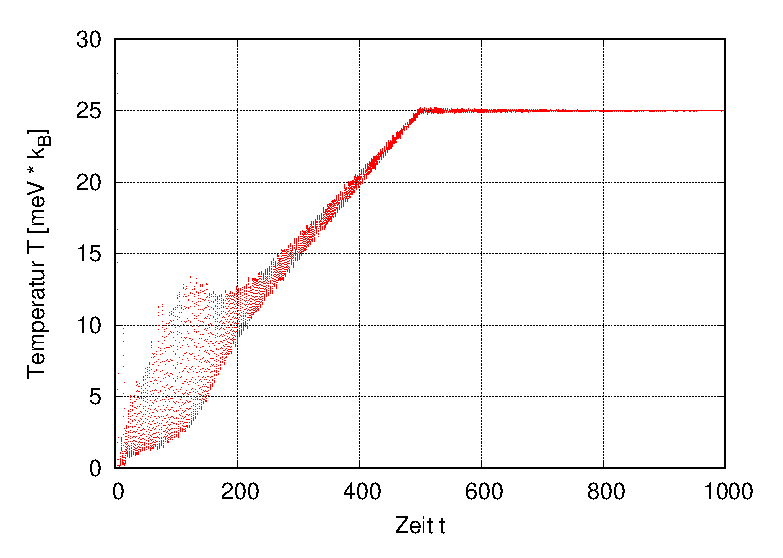
\includegraphics[width=0.9\textwidth]{chapter/main/single/plt/equilibration/thermostat.eps}
			\caption{Der Aufheizprozess mit vorgegebener Temperatur. Die Fluktuationen werden
			mit fortschreitender Zeit geringer.}
			\label{fig:thermostat}
		\end{figure}

		Abbildung \ref{fig:thermostat} zeigt das Aufheizen einer würfelförmigen Probe mithilfe des
		in IMD implementierten Nosé-Hoover-Thermostats. Während die Temperatur am Anfang trotz
		Vorgabe noch schwankt, vermindert sich dieser Effekt mit der Zeit. Ab ungefähr 800
		Zeiteinheiten sind die Fluktuationen in etwa konstant.

		\begin{figure}[!ht]
			\centering
			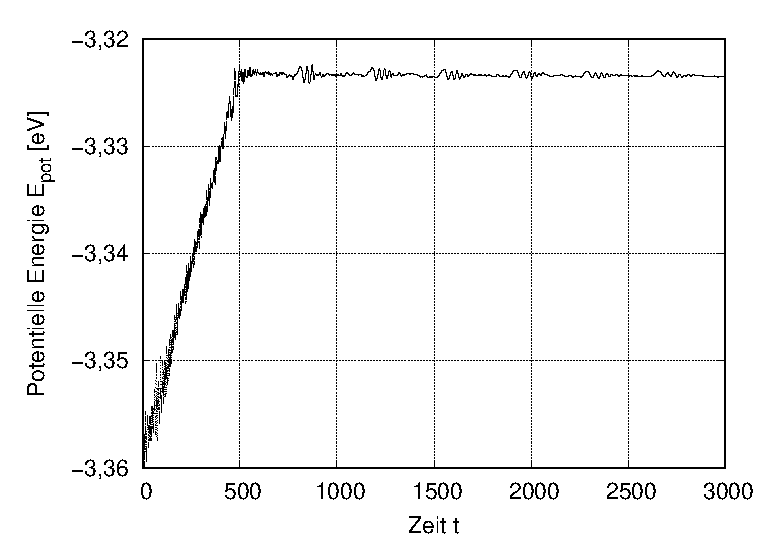
\includegraphics[width=0.9\textwidth]{chapter/main/single/plt/equilibration/thermostat_pot.eps}
			\caption{Die potentielle Energie zeigt einen zur Temperatur proportionalen Verlauf}
			\label{fig:thermostat_pot}
		\end{figure}

		Wie allerdings in Abbildung \ref{fig:thermostat_pot} zu sehen ist, verhält sich die
		potentielle Energie proportional zum Temperaturverlauf. Von daher ist es ratsam nach dem
		Aufheizen eine NVE-Simulation bis zum Equilibrium durchzuführen.

	\subsection{Erzeugen einer Kugelprobe}
		Üblicherweise sind Proben quaderförmig und bilden durch \emph{periodischen Randbedingungen}
		(\emph{PBC}) ein Gitter, welches teilweise Eigenschaften eines unendlich ausgedehnten
		Gitters imitiert. Im Rahmen dieser Arbeit sind jedoch Kugelformen unter der Einwirkung von
		Gravitation interessant, da sie so den Pulverpartikeln beim SLM-Verfahren sehr ähnlich
		sind. Die einfachste Methode zum Erzeugen einer solchen Probe ist die Wahl eines
		entsprechenden Gitterausschnitts, wobei die umliegenden Teilchen entfernt werden.
		Hierbei gilt zu beachten, dass die Kugel erst nach der homogenen Deformation freigestellt
		wird. Das hat den Grund, dass eine homogene Deformation das gesamte Teilchensystem
		skaliert. Ist der Radius der Kugel sehr genau bemaßt, ändert er sich signifikant während
		dieses Prozesses. Wichtig ist für die nachfolgenden Equilibrierungsschritte auf jeden
		Fall, dass diese nun unter Einfluss der Gravitation mit ausreichend Equilibrierungszeit
		erfolgen. So wird gewährleistet, dass die Kugel etwas absackt und sich somit in ihre der
		Form entsprechenden Ruhelage begibt. Abbildung \ref{fig:equilibrated_sample} zeigt dabei
		die Ruhelage eines kugelförmigen Gitterausschnitts mit einem Durchmesser von
		\SI{400}{\angstrom}. Zwischen fixiertem Boden und beweglicher Kugel vergrößert sich die
		Kontaktfläche durch die Wirkung der Gravitation.

		Es ist allgemein empfehlenswert, wenn die Kugel nicht direkt in den Einflussbereich der
		PBC positioniert wird. Um eine derartige Selbstbeeinflussung zu verhindern könnten die PBC
		deaktiviert werden, jedoch stellten diese sich für die Erstellung problemverwandter Proben
		als nützlich heraus. So kann beispielsweise eine Simulationsbox mehrfach
		hintereinanderkopiert werden, um eine Reihe an Kugeln zu erhalten. Sofern diese
		ursprüngliche Probe mit PBC equilibriert wurde, sind randübergreifende Aspekte wie der
		Boden nahtlos wiederholbar, wodurch das System nicht erneut equilibriert werden muss. Das
		spart vor allem bei größeren Proben Zeit.

		\begin{figure}[!ht]
			\centering
			\includegraphics[width=\textwidth]{chapter/main/single/img/equilibrated_sphere.zoom.png}
			\caption{Eine vollständig equilibrierte Kugel aus Aluminiumatomen (grün) auf einem
			festen, unbeweglichen Untergrund (rot) vergrößert die Kontaktfläche unter dem eigenen
			Gewicht}
			\label{fig:equilibrated_sample}
		\end{figure}


\section{Kalibrierung der Laserleistung bei fester Lasergeschwindigkeit}
\todo[color=green]{Vielleicht geschmolzenen Anteil gehen? Eventuell Kapitelaufteilung in verschiedene Leistungen?}

\section{Verhalten bei halbierter Lasergeschwindigkeit}
